\section{Fonctionnalités}

\begin{frame}
\frametitle{Les grandes familles de fonctionnalités dans l'OTB (forcément incomplètes)}

\begin{block}{Pré-traitements}
\begin{itemize}
\item Calibration radiométrique, ortho-rectification, reprojection (raster et vecteur), pan-sharpening, stéréo-rectification,
\item Capteurs supportés: Sentinels, Pléiades, SPOT6, SPOT5, capteurs DigitalGlobe
\item Modélisation géométrique fournie par OSSIM, support de MNT SRTM ou GeoTIFF
\end{itemize}
\end{block}

\begin{block}{Manipulation d'images et de vecteurs}
\begin{itemize}
\item Formats supportés par Gdal (raster et vecteur), conversion raster/vecteur
\item Extraction de ROI, de bandes spectrales, concaténation ou séparation des bandes spectrales,
\item calcul mathématiques entre bandes, color mapping, optimisation du contraste
\item Filtrage linéaire, morphologie mathématique,
\end{itemize}
\end{block}
\end{frame}

\begin{frame}
\frametitle{Les grandes familles de fonctionnalités dans l'OTB (forcément incomplète)}

\begin{block}{Détection d'éléments saillants et calcul de primitives}
\begin{itemize}
\item Détection de contours, points d'intérêt SIFT et SURF, lignes, angles droits
\item Indices radiométriques, indices de textures (Haralick, SFS, PanTex)
\item Descripteurs statistiques locaux (moments de Flusser, HOG)
\item Matching de points d'intérêts
\end{itemize}
\end{block}

\begin{block}{Détection de changement}
\begin{itemize}
\item Algorithme classique avec métrique de comparaison d'images,
\item Algorithme MAD (Multivariate Alteration Detector)
\end{itemize}
\end{block}

\begin{block}{Réduction de la dimension, traitement hyperspectraux}
\begin{itemize}
\item Réduction de la dimension: PCA, NAPCA, ICA, MAF \ldots
\item Estimation de la dimension et extraction des pixels purs: algorithme VCA
\end{itemize}
\end{block}

\end{frame}

\begin{frame}
\frametitle{Les grandes familles de fonctionnalités dans l'OTB (forcément incomplète)}
\begin{block}{Segmentation}
\begin{itemize}
\item Algorithmes de segmentation Connected Components, MeanShift, Ligne de partage des eaux
\item Méthodologie pour une application large échelle,
\item Représentation vectorielles et raster des résultats, avec capacités d'analyse objet
\end{itemize}
\end{block}

\begin{block}{Classification}
\begin{itemize}
\item Supervision et classification d'images avec 9 algorithmes au choix (dont SVM et forêts aléatoires)
\item Fusion et régularisation de cartes de classification
\item Clustering de type K-Means ou carte de Kogonen
\item Classification objets (segments issus d'une segmentation)
\end{itemize}
\end{block}

\end{frame}

\vspace*{-6.5mm}
\begin{frame}[plain]
\hspace*{-11mm}
    \includegraphics[keepaspectratio,height=1.1\paperheight]{images/mayotte2012.png}
\end{frame}

\vspace*{-6.5mm}
\begin{frame}[plain]
\hspace*{-11mm}
    \includegraphics[keepaspectratio,height=1.1\paperheight]{images/mayotte2013.png}
\end{frame}

\vspace*{-6.5mm}
\begin{frame}[plain]
\hspace*{-11mm}
    \includegraphics[keepaspectratio,height=1.1\paperheight]{images/mayotte_mad.png}
\end{frame}

\vspace*{-6.5mm}
\begin{frame}[plain]
\hspace*{-11mm}
\includegraphics[keepaspectratio,height=1.1\paperheight]{images/saint_paul_lsd.png}
\end{frame}

\vspace*{-6.5mm}
\begin{frame}[plain]
\hspace*{-11mm}
    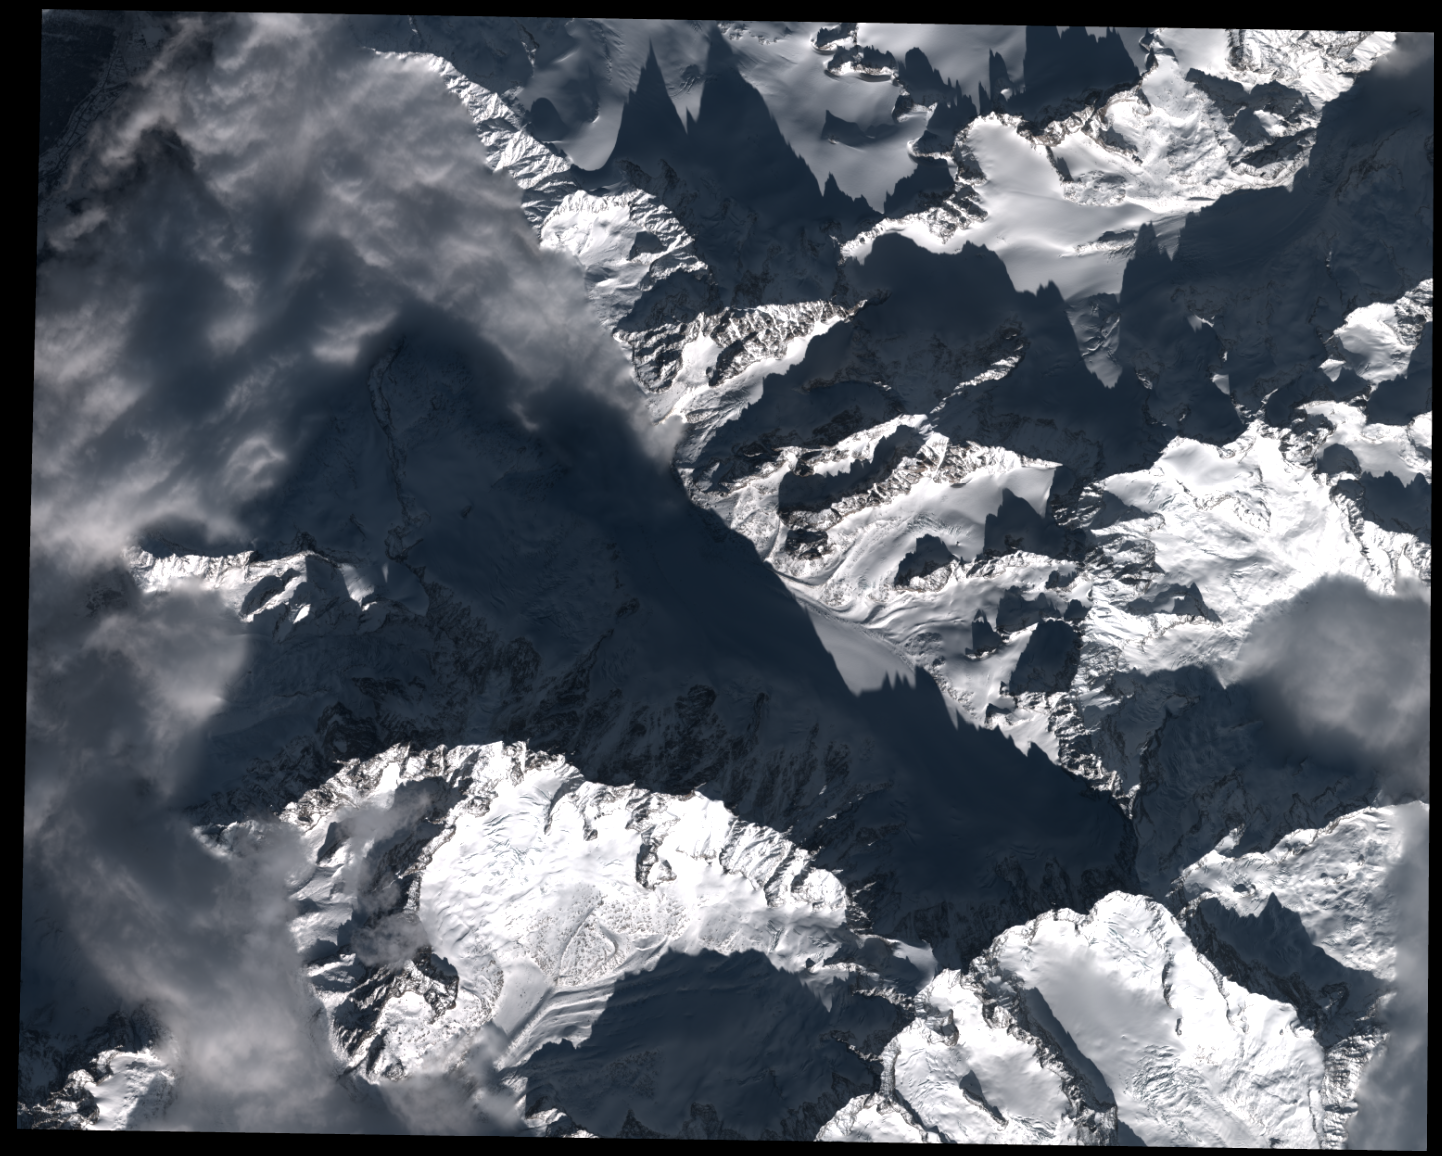
\includegraphics[keepaspectratio,width=1.005\paperwidth,height=1.1\paperheight]{images/argentiere_left.png}
\end{frame}

\vspace*{-6.5mm}
\begin{frame}[plain]
\hspace*{-11mm}
    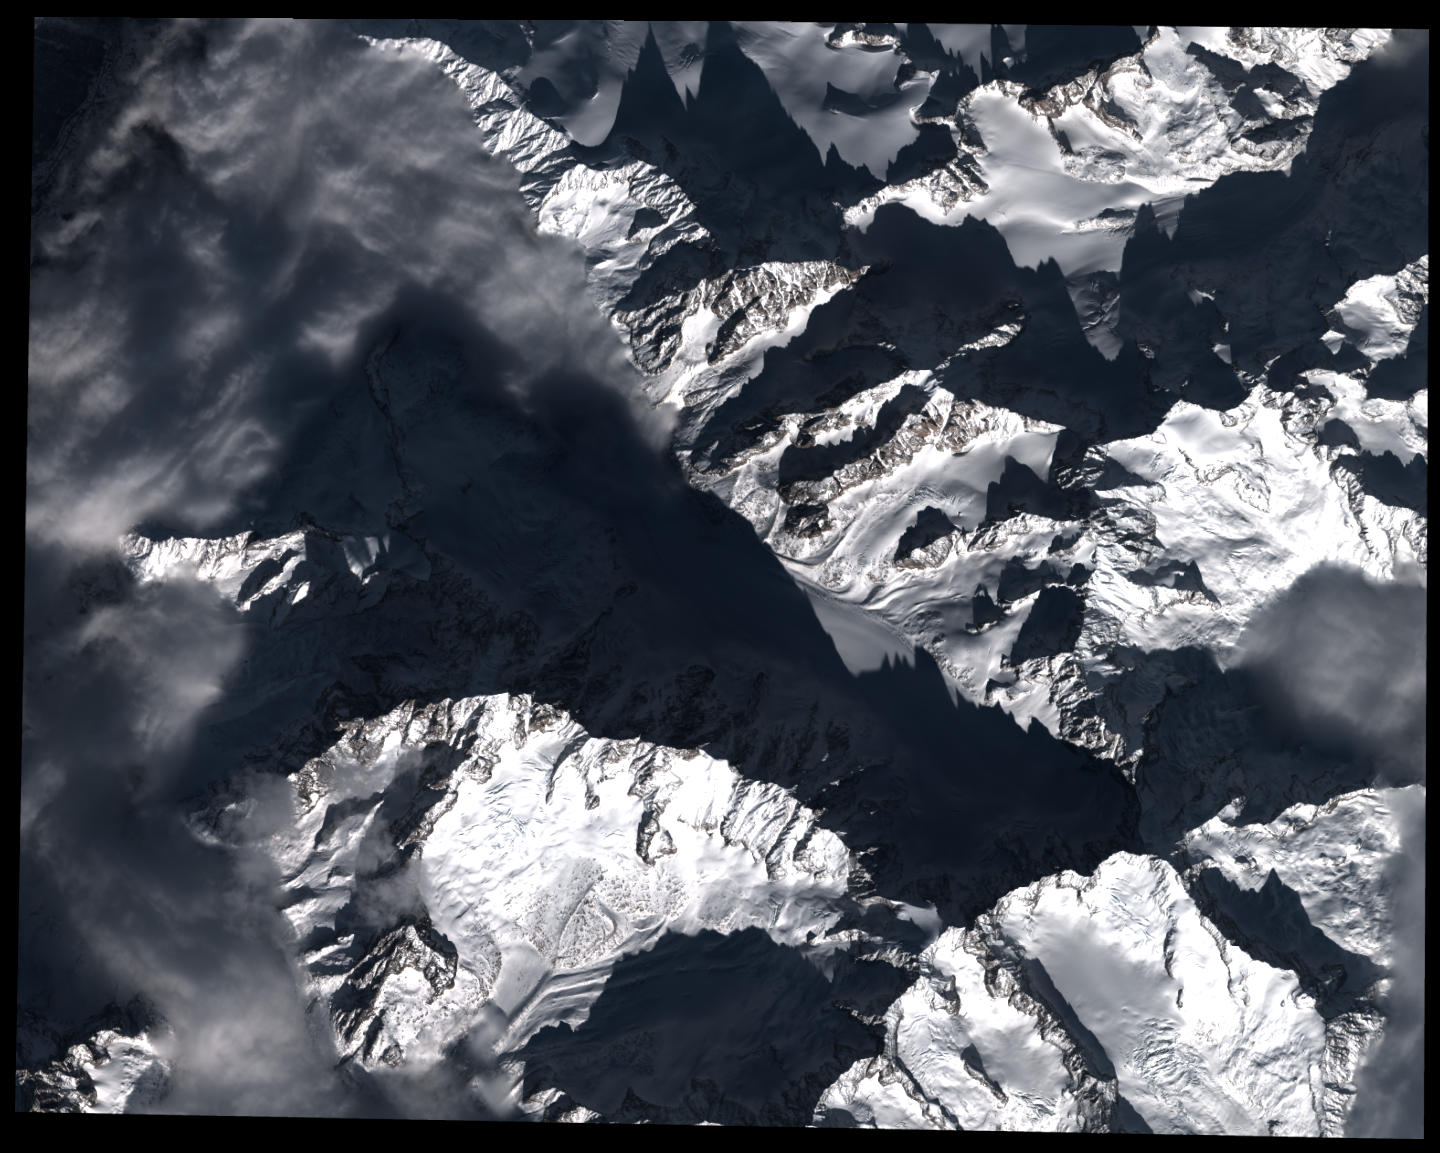
\includegraphics[keepaspectratio,width=1.005\paperwidth,height=1.1\paperheight]{images/argentiere_right.png}
\end{frame}

\vspace*{-6.5mm}
\begin{frame}[plain]
\hspace*{-11mm}
    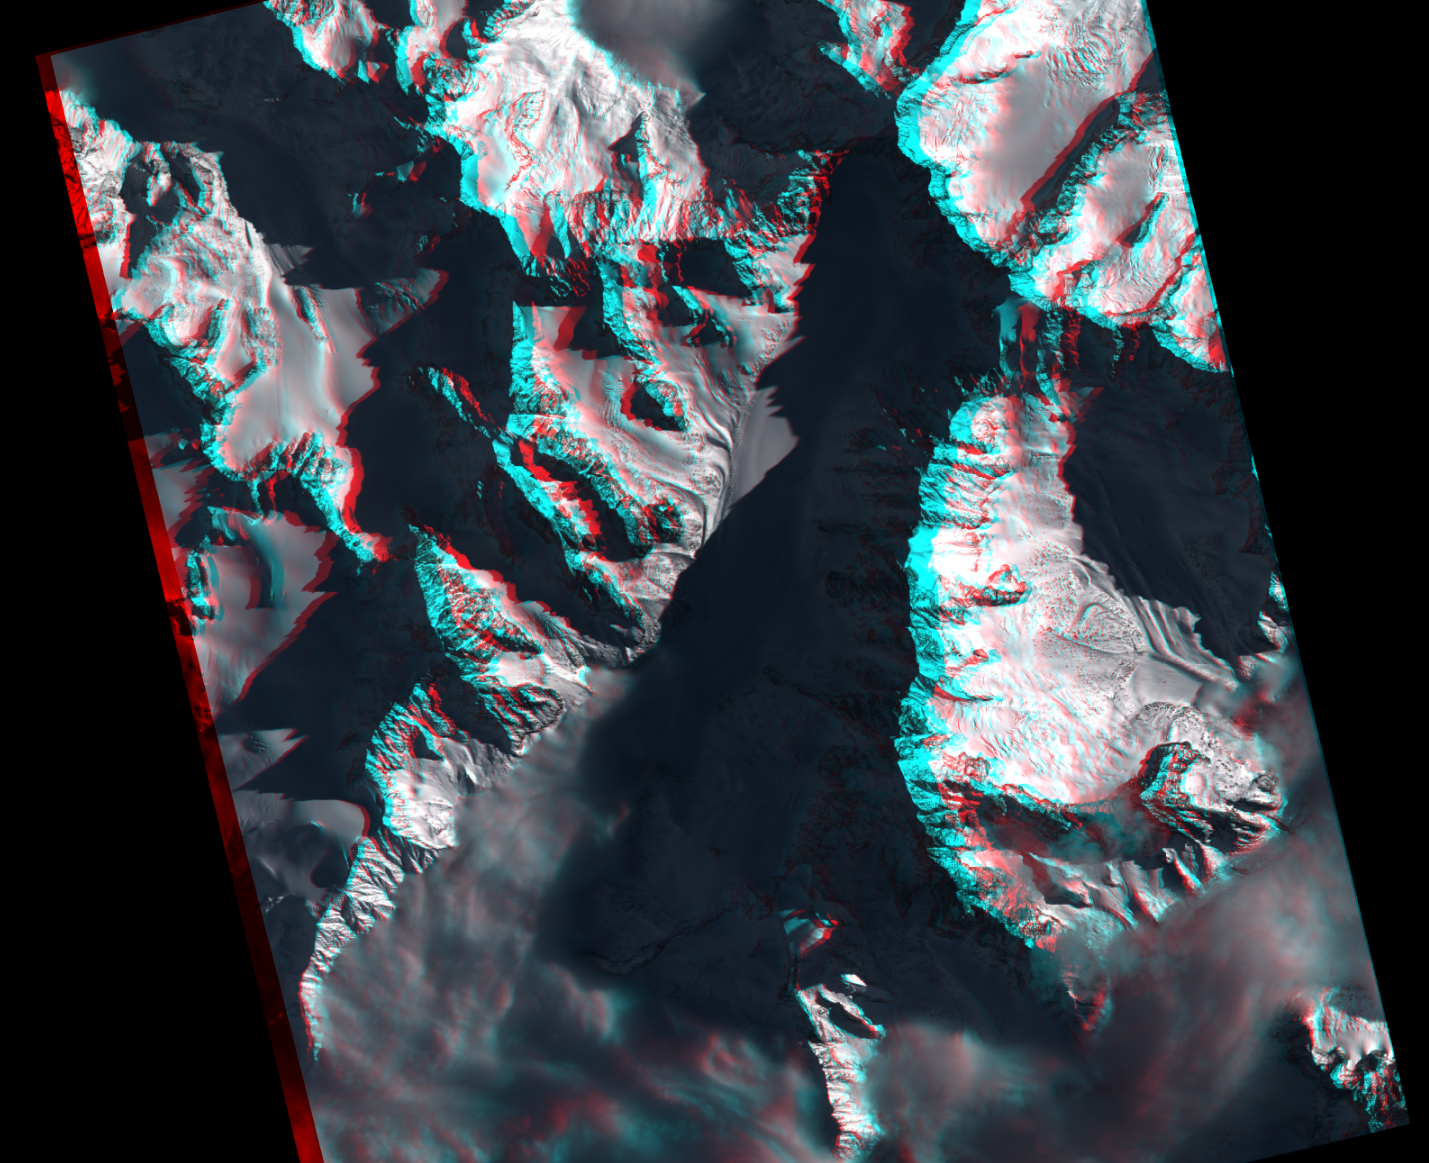
\includegraphics[keepaspectratio,width=1.005\paperwidth,height=1.1\paperheight]{images/argentiere_anaglyphe.png}
\end{frame}

\vspace*{-6.5mm}
\begin{frame}[plain]
\hspace*{-11mm}
    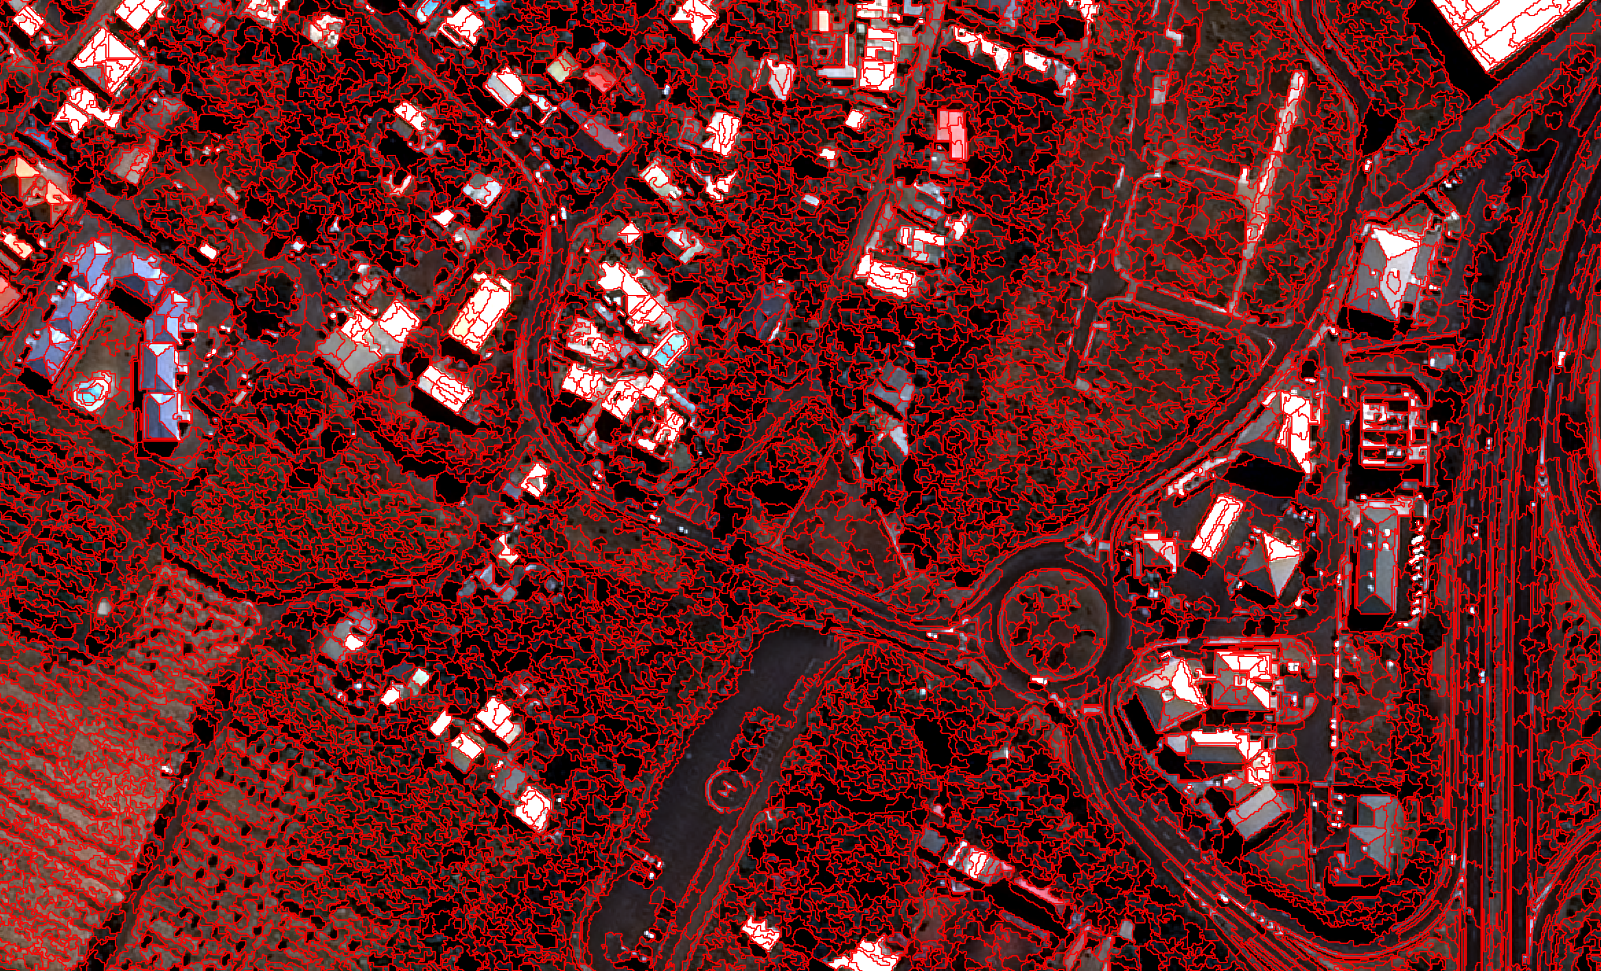
\includegraphics[keepaspectratio,height=1.1\paperheight]{images/segmentation.png}
\end{frame}

\vspace*{-6.5mm}
\begin{frame}[plain]
\hspace*{-11mm}
    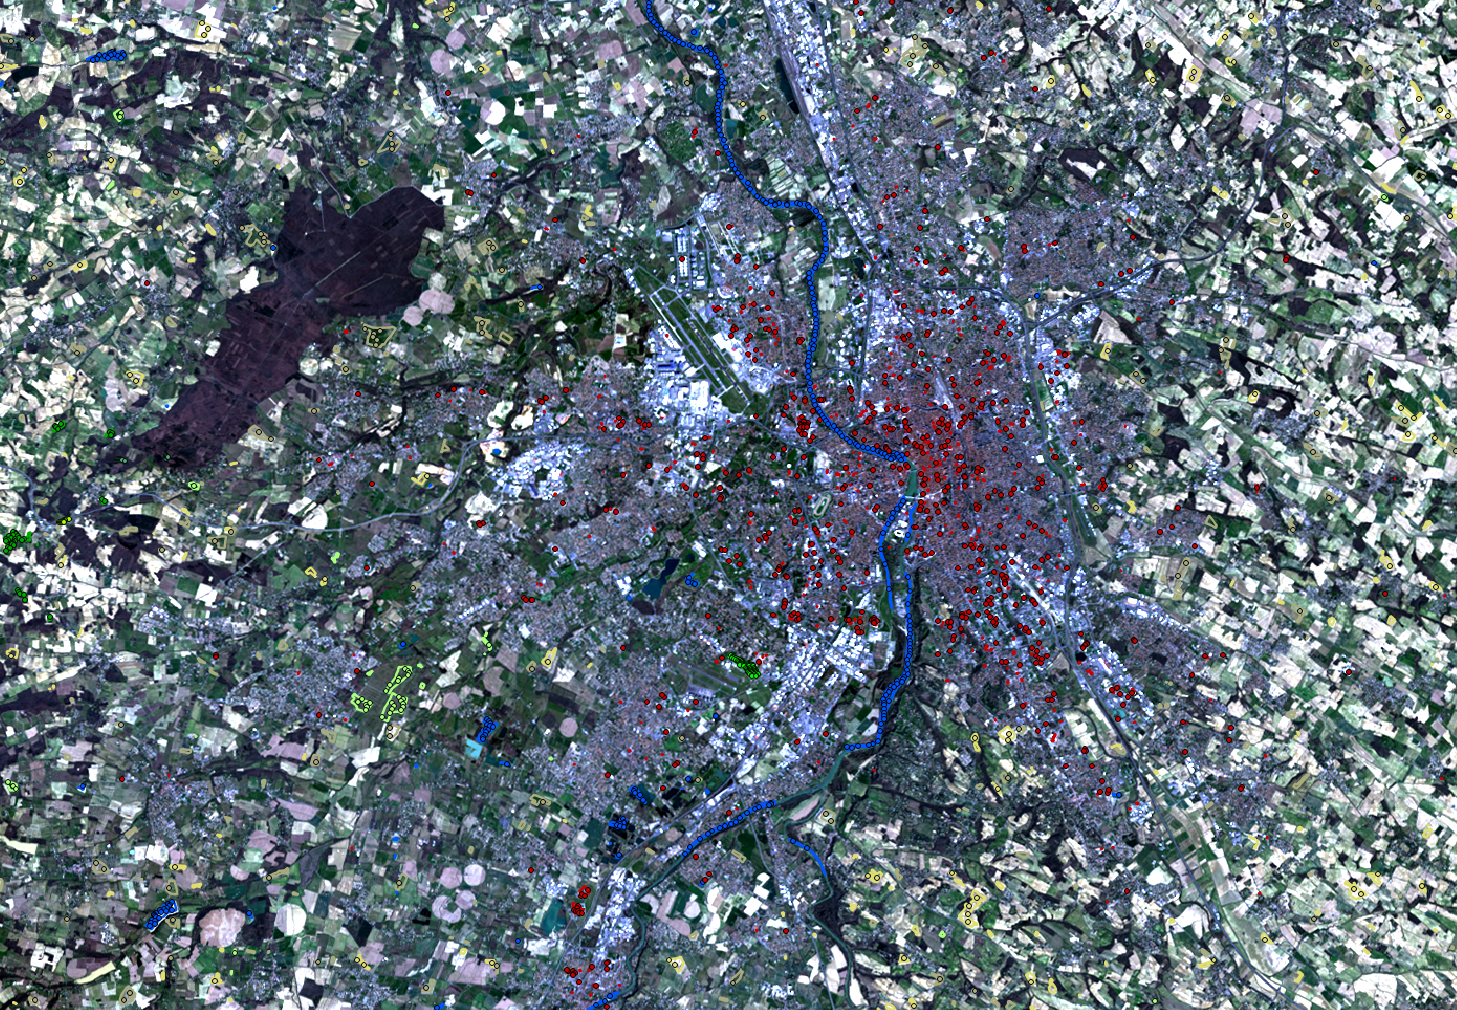
\includegraphics[keepaspectratio,height=1.1\paperheight]{../../Courses/org/WorkshopGuide/Images/samples_selection.png}
\end{frame}


\vspace*{-6.5mm}
\begin{frame}[plain]
\hspace*{-11mm}
    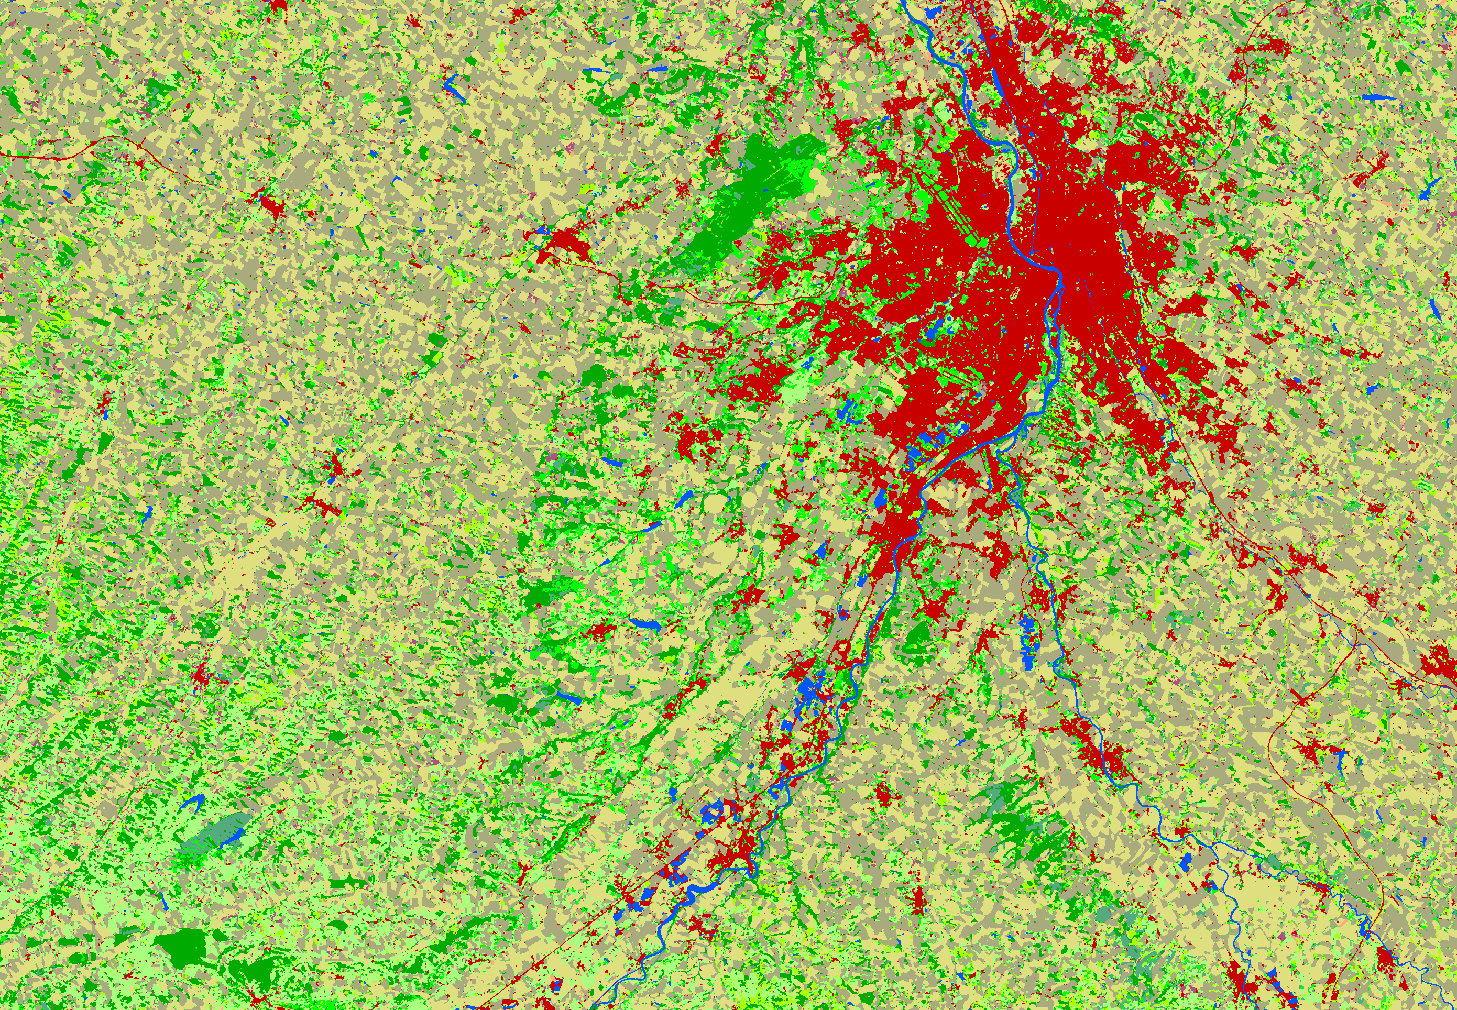
\includegraphics[keepaspectratio,height=1.1\paperheight]{../../Courses/org/WorkshopGuide/Images/final_classification.png}
\end{frame}

\vspace*{-6.5mm}
\begin{frame}[plain]
\hspace*{-11mm}
    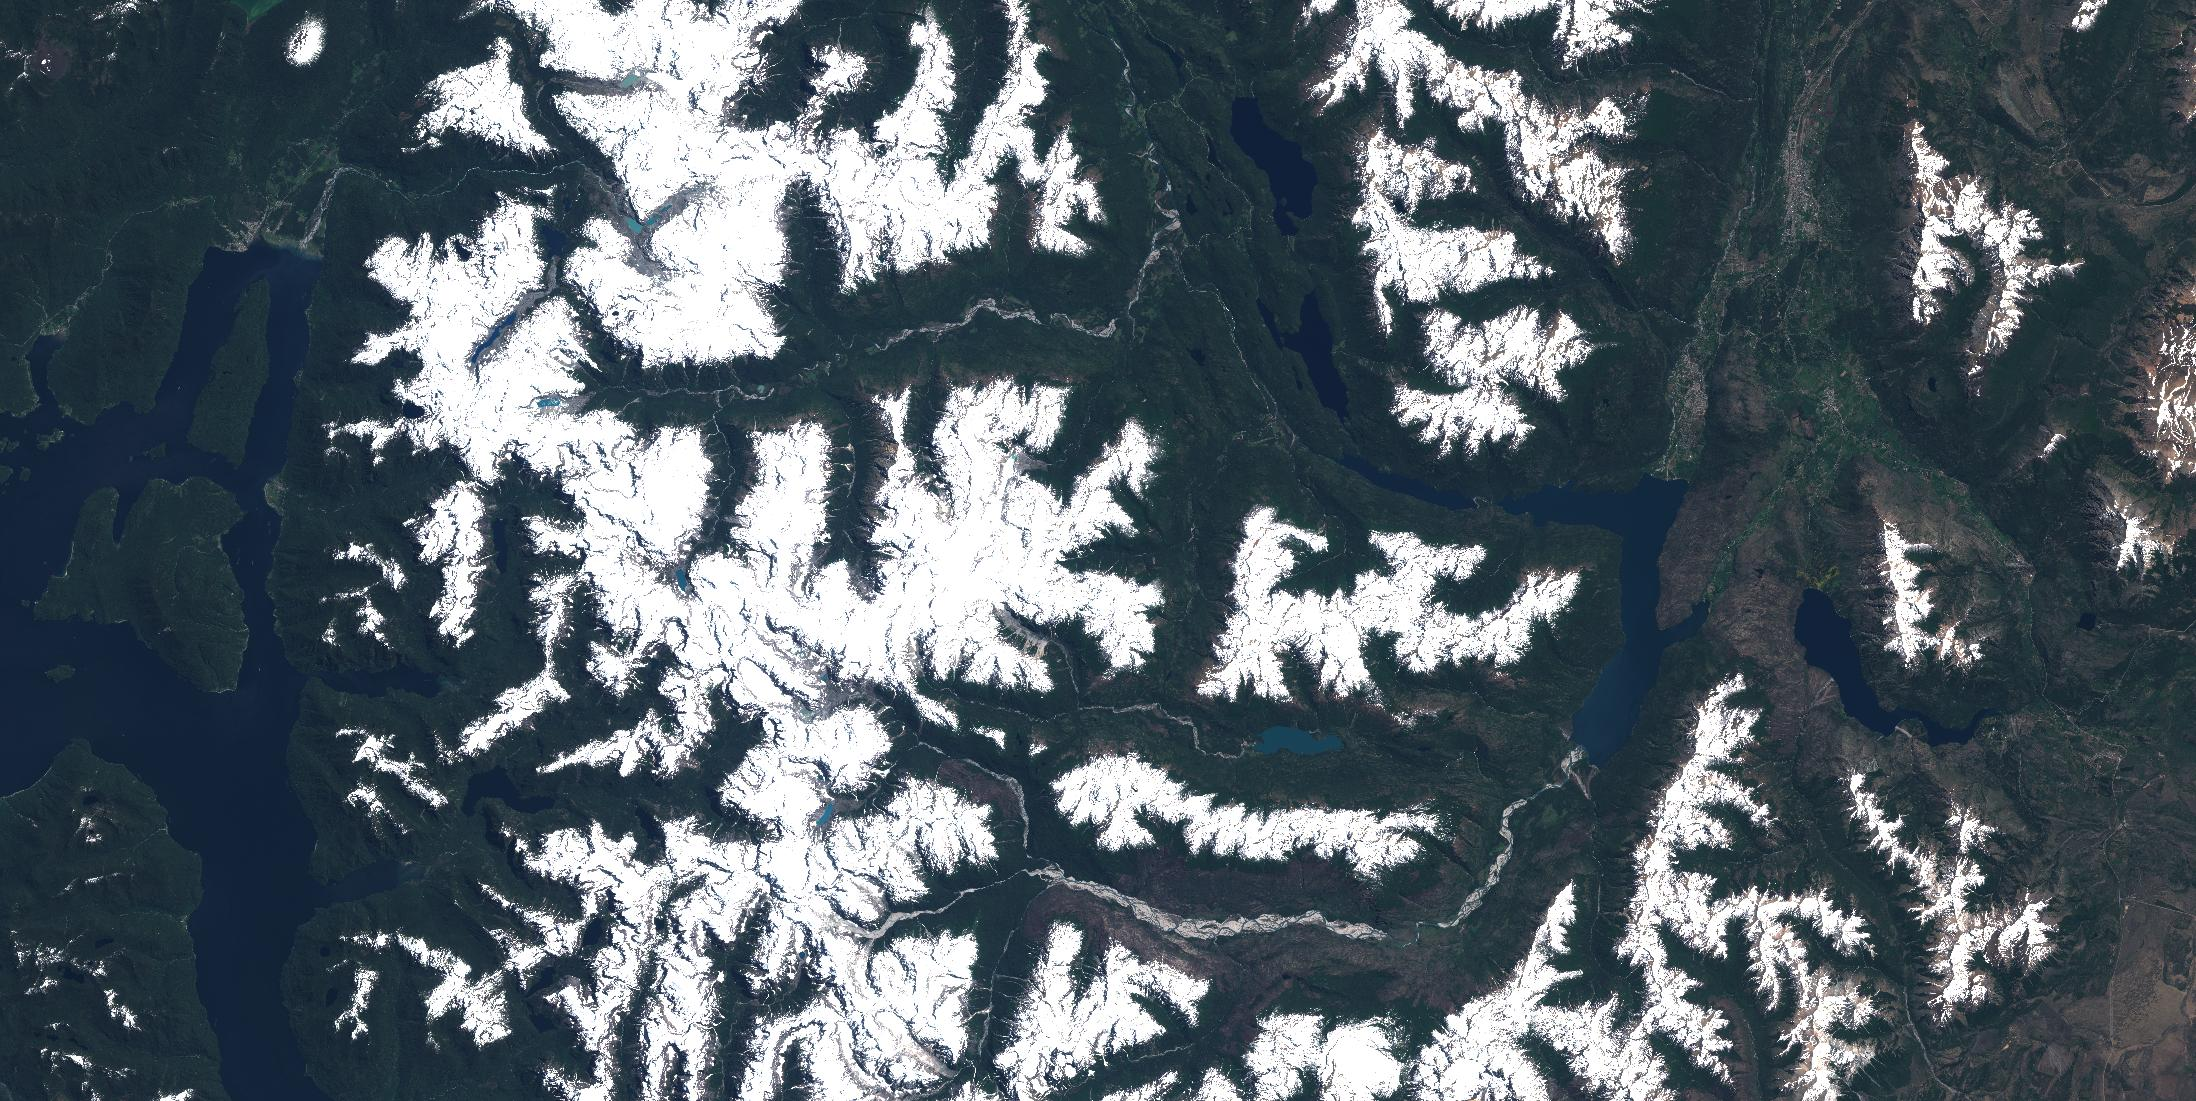
\includegraphics[keepaspectratio,height=1.1\paperheight]{images/imag4tci.jpg}
\end{frame}

\vspace*{-6.5mm}
\begin{frame}[plain]
\hspace*{-11mm}
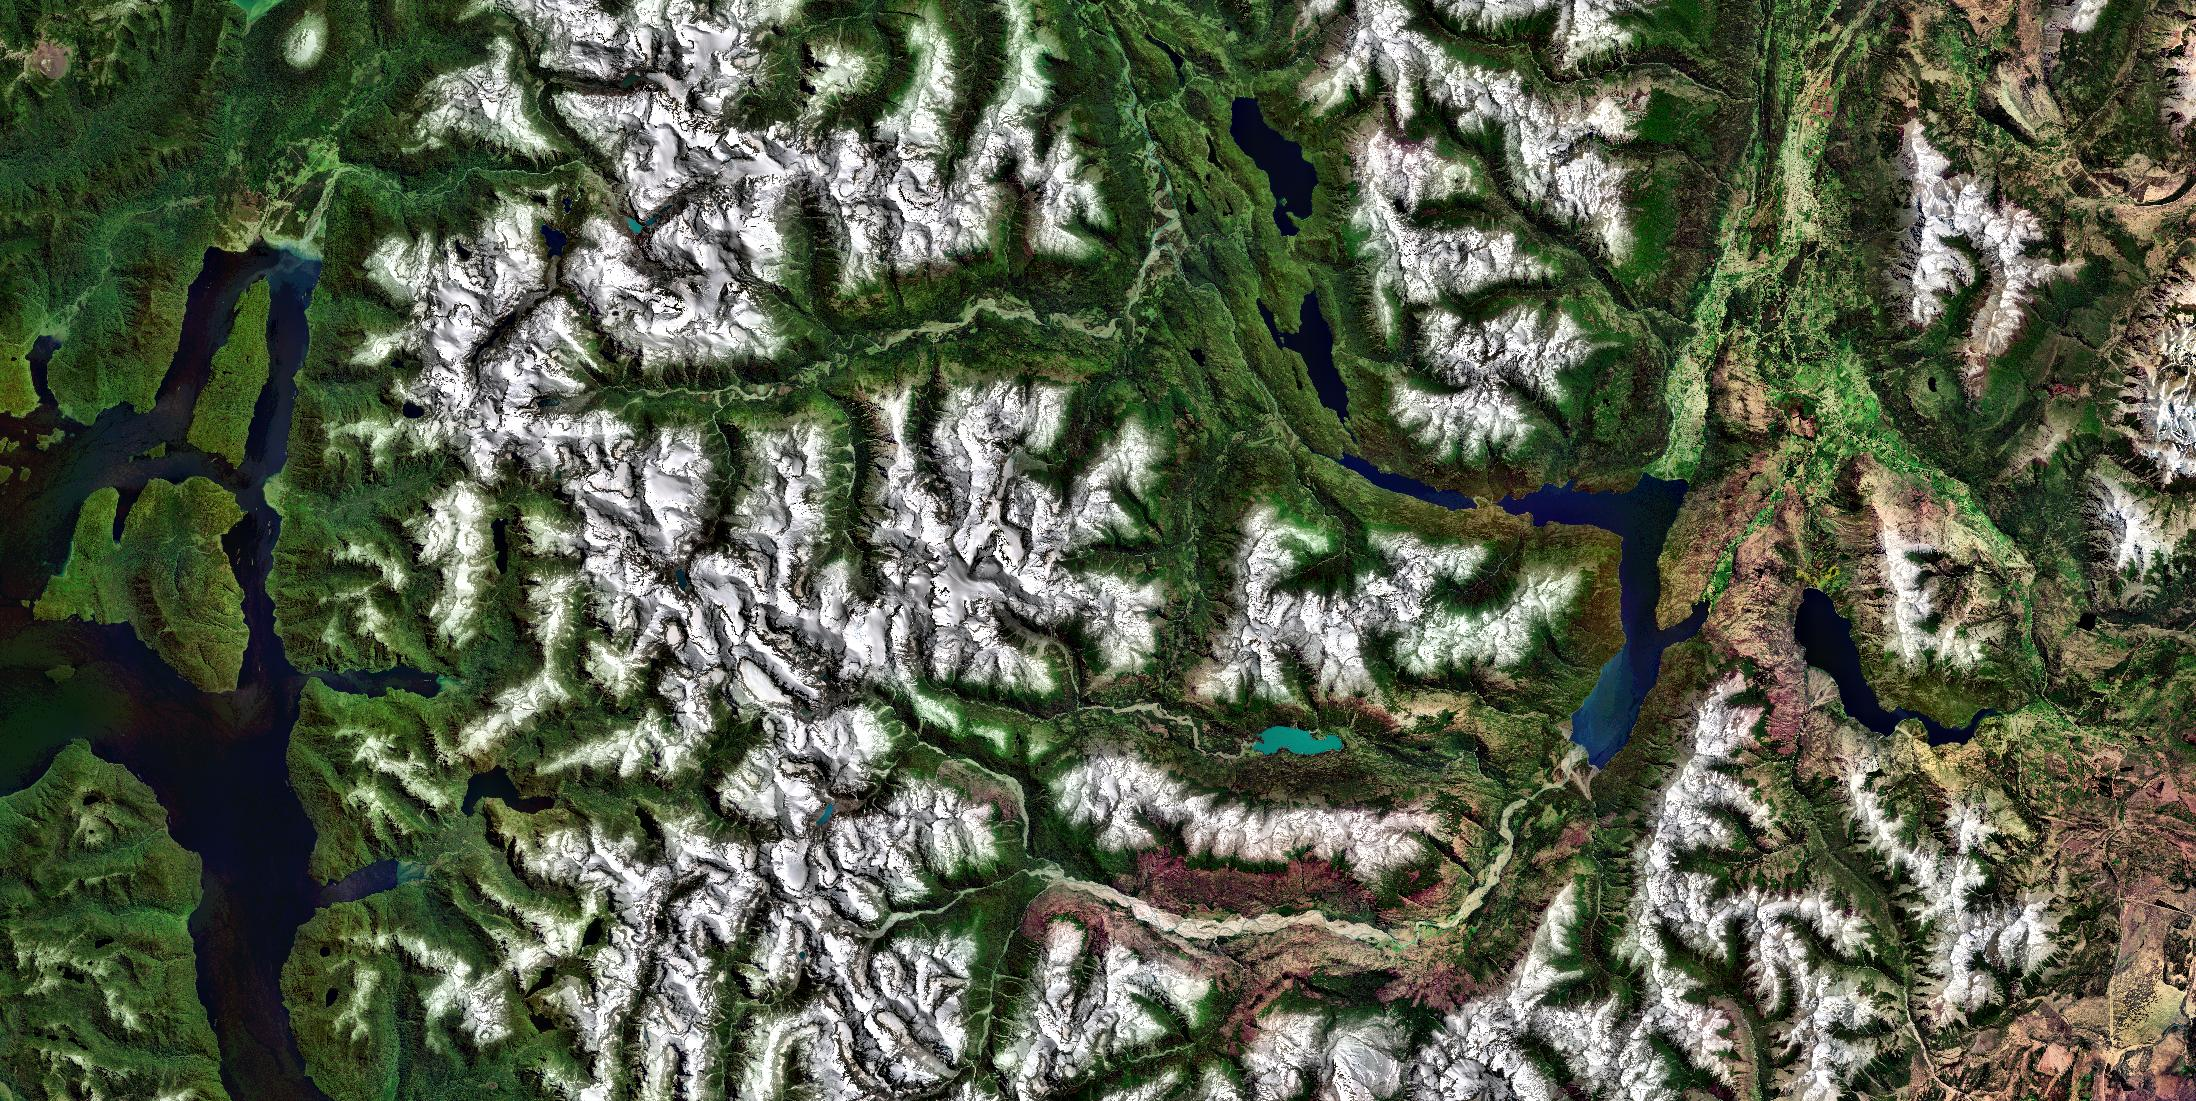
\includegraphics[keepaspectratio,height=1.1\paperheight]{images/image4_glob_each_lim20_8b_sub.jpg}
\end{frame}
